\chapter{Listas Baseadas em Array}
\chaplabel{arrays}

Neste capítulo, estudaremos as implementações das interfaces #Lista# e #Fila# 
nas quais os dados subjacentes são armazenados em um array, chamado de 
\emph{array de base}.
\index{backing array}%
A tabela a seguir resume os tempos de execução das operações das 
estruturas de dados apresentadas neste capítulo:
\newlength{\tabsep}
\setlength{\tabsep}{\itemsep}
\addtolength{\tabsep}{\parsep}
\addtolength{\tabsep}{-2pt}
\begin{center}
\vspace{\tabsep}
\begin{tabular}{|l|l|l|} \hline
 & #get(i)#/#set(i,x)# & #add(i,x)#/#remove(i)# \\ \hline
#ArrayStack# & $O(1)$ & $O(#n#-#i#)$ \\
#ArrayDeque# & $O(1)$ & $O(\min\{#i#,#n#-#i#\})$ \\
#DualArrayDeque# & $O(1)$ & $O(\min\{#i#,#n#-#i#\})$ \\
#RootishArrayStack# & $O(1)$ & $O(#n#-#i#)$ \\ \hline
\end{tabular}
\vspace{\tabsep}
\end{center}
Estruturas de dados que funcionam armazenando dados em um único array 
têm muitas vantagens e limitações em comum:
\index{arrays}%
\begin{itemize}
  \item Os arrays oferecem acesso com tempo constante a qualquer valor 
  no array. Isto é o que permite que #get (i) # e #set (i, x) # sejam 
  executados em tempo constante.

  \item Arrays não são muito dinâmicos. Adicionar ou remover um elemento 
  perto do meio de uma lista significa que um grande número de elementos 
  no array precisa ser deslocado para abrir espaço para o elemento 
  recém-adicionado ou para preencher a lacuna criada pelo elemento 
  excluído. É por isso que as operações #add(i, x)# e #remove(i)# 
  têm tempos de execução que dependem de #n# e #i#.

  \item Arrays não podem expandir ou encolher. Quando o número de elementos 
  na estrutura de dados excede o tamanho do array de base, um novo array precisa 
  ser alocado e os dados do array antigo precisam ser copiados para o novo 
  array. Esta é uma operação cara.
\end{itemize}
O terceiro ponto é importante. Os tempos de execução citados na tabela 
acima não incluem o custo associado ao crescimento e ao encolhimento do 
array de base. Veremos que, se cuidadosamente gerenciado, o custo de 
crescer e encolher o array de base não aumenta muito o custo de uma 
operação \emph{média}. Mais precisamente, se começarmos com uma estrutura 
de dados vazia e executarmos qualquer sequência de $m$ operações #add(i, x)# 
ou #remove (i)#, então o custo total do crescimento e encolhimento do 
array de base, sobre a sequência inteira de $m$ operações é $O(m)$. 
Embora algumas operações individuais sejam mais caras, o custo amortizado, 
quando amortizado em todas as operações de $m$, é de apenas $O(1)$ por operação.

\cpponly{
Neste capítulo, e ao longo deste livro, será conveniente ter arrays que 
acompanhem o seu tamanho. Os arrays usuais de C++ não fazem isso, 
então definimos uma classe, #array#, que mantém o controle de seu comprimento. 
A implementação desta classe é simples. Ela é implementada como um array padrão 
de C++ padrão, #a#, e um inteiro, #length#:} 
\cppimport{ods/array.a.length}
\cpponly{
O tamanho de um #array# é especificado no momento da criação:
}
\cppimport{ods/array.array(len)}
\cpponly{Os elementos de uma array podem ser indexados:}
\cppimport{ods/array.operator[]}
\cpponly{Finalmente, quando um array é atribuído a outra, esta é 
apenas uma manipulação de ponteiro que leva tempo constante:}
\cppimport{ods/array.operator=}

\section{#ArrayStack#: Operações Rápidas de Pilha usando um Array}
\seclabel{arraystack}

\index{ArrayStack@#ArrayStack#}%
Um #ArrayStack# implementa a interface de lista usando um array #a#, 
chamado de \emph{array de base}. O elemento de lista com índice #i# é 
armazenado em #a[i]#. Na maioria das vezes, #a# é maior do que o 
estritamente necessário, então um número inteiro #n# é usado para manter 
o controle do número de elementos realmente armazenados em #a#. Desta 
forma, os elementos da lista são armazenados em #a[0]#,\ldots,#a[n-1]# 
e, sempre, $#a.length# \ge #n#$.

\codeimport{ods/ArrayStack.a.n.size()}

\subsection{O Básico}

Acessar e modificar os elementos de um #ArrayStack# usando #get(i)# 
e #set(i,x)# é trivial. Depois de realizar qualquer verificação de 
limites necessária, simplesmente retornamos ou atribuímos, 
respectivamente, #a[i]#.

\codeimport{ods/ArrayStack.get(i).set(i,x)}

As operações de adicionar e remover elementos de um #ArrayStack# são 
ilustradas na \figref{arraystack}. Para implementar a operação #add(i, x)#, 
verificamos primeiro se #a# já está cheio. Em caso afirmativo, chamamos 
o método #resize()# para aumentar o tamanho de #a#. Como #resize()# será 
implementado discutiremos mais tarde. Por enquanto, basta saber que, 
após uma chamada a #resize()#, podemos ter certeza de que $#a.length#
> #n#$. Com isto resolvido, agora deslocamos os elementos 
$#a[i]#,\ldots,#a[n-1]#$ uma posição à direita para abrir espaço 
para #x#, fazemos #a[i]# igual a #x# e incrementamos #n#.

\begin{figure}
  \begin{center}
    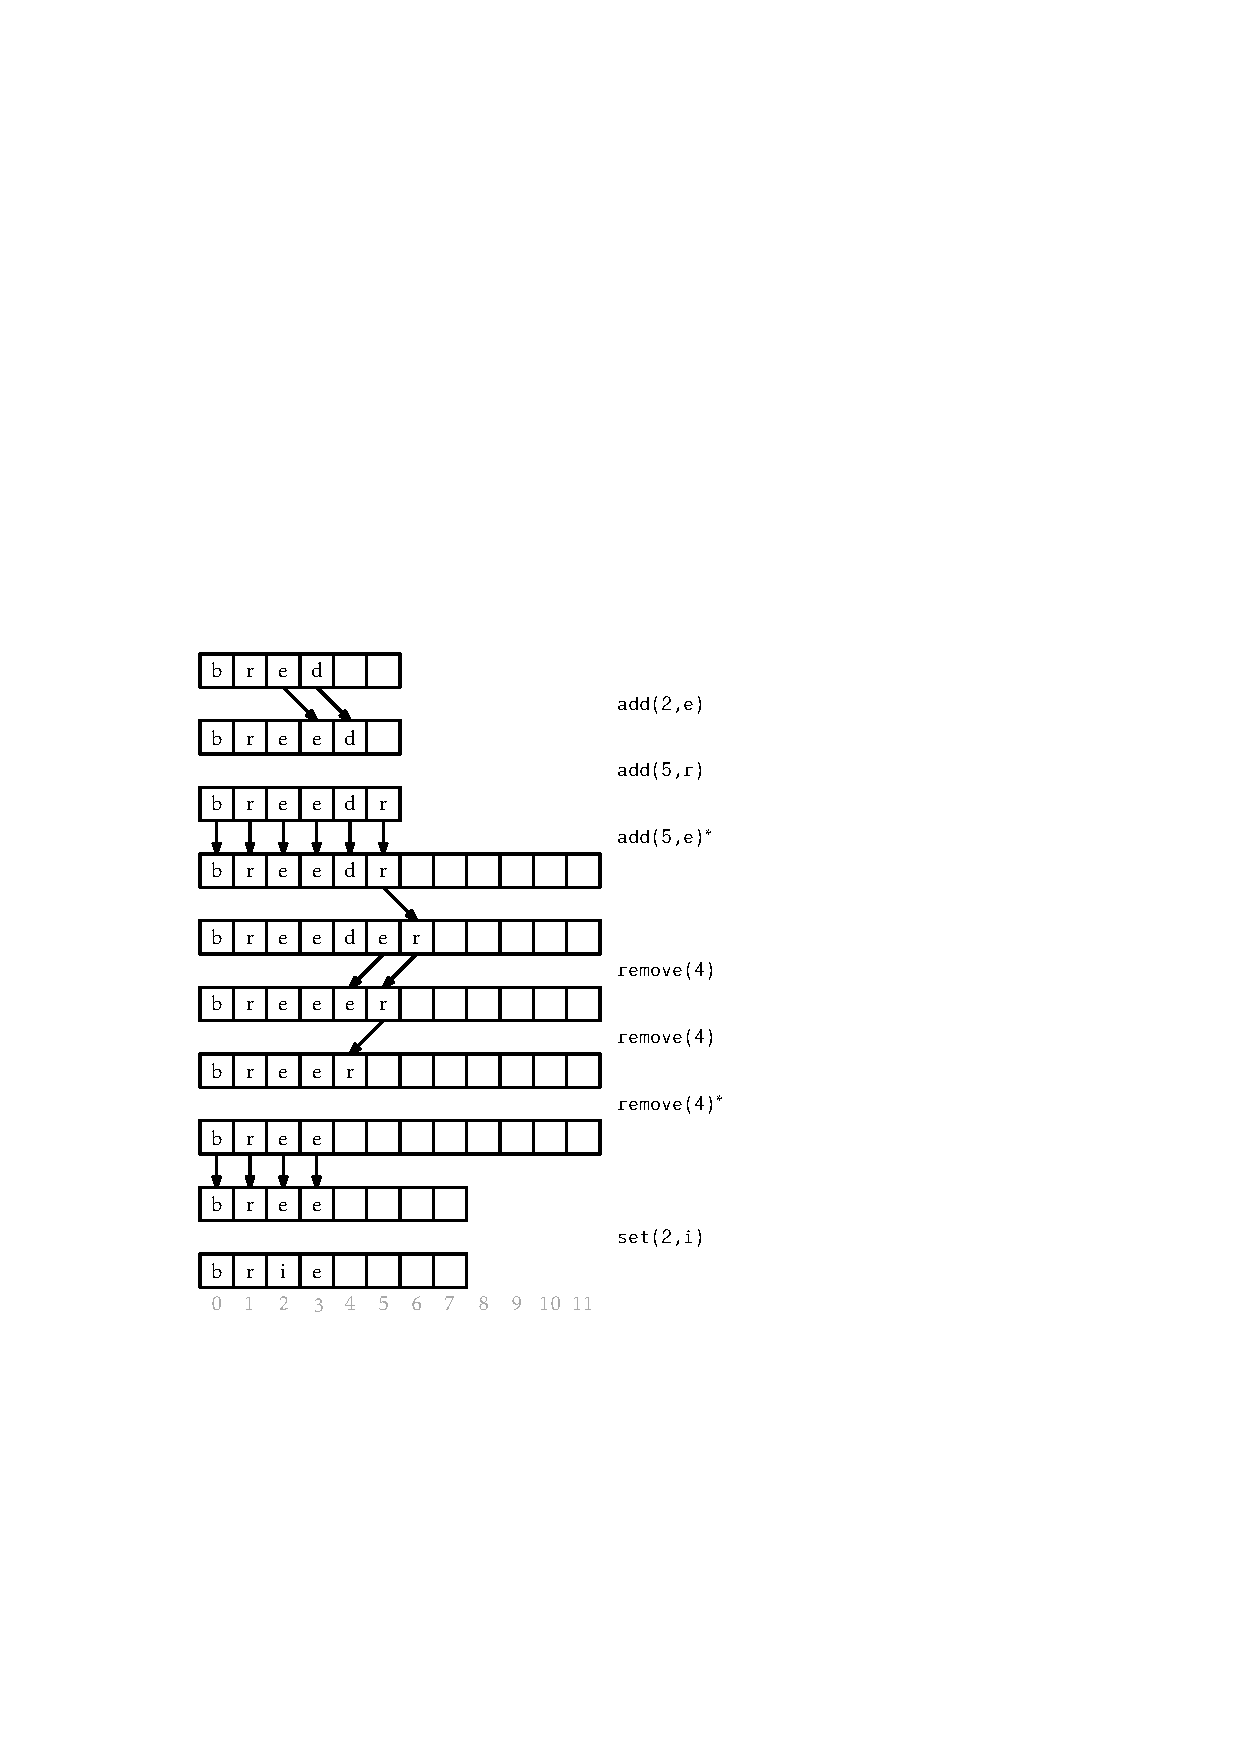
\includegraphics[scale=0.90909]{figs/arraystack}
  \end{center}
  \caption[Adicionando a um ArrayStack]{Uma sequência de operações 
  #add(i,x)# e #remove(i)# em um #ArrayStack#. As setas indicam 
  elementos que estão sendo copiados. As operações que resultam 
  em uma chamada para #resize()# são marcadas com um asterisco.}
  \figlabel{arraystack}
\end{figure}

\codeimport{ods/ArrayStack.add(i,x)}
Se ignorarmos o custo da possível chamada para #resize()#, então o 
custo da operação #add(i,x)# é proporcional ao número de elementos 
que temos de deslocar para criar espaço para #x#. Portanto, o custo 
desta operação (ignorando o custo de redimensionar #a#) é $O(#n#-#i#)$.

Implementar a operação #remove(i)# é semelhante. Deslocamos os elementos 
$#a[i+1]#,\ldots,#a[n-1]#$ uma posição para a esquerda (sobrescrevendo 
#a[i]#) e diminuindo o valor de #n#. Depois de fazer isso, verificamos 
se #n# está ficando muito menor que #a.length# verificando se 
$#a.length# \ge 3#n#$. Em caso afirmativo, chamamos #resize()# para 
reduzir o tamanho de #a#.

\codeimport{ods/ArrayStack.remove(i)}
% TODO: Add shifting figure
Se ignorarmos o custo do método #resize()#, o custo de uma operação 
#remove(i)# é proporcional ao número de elementos que deslocamos, que 
é $O(#n#-#i#)$.

\subsection{Crescendo e Encolhendo}

O método #resize()# é bastante direto; ele aloca um novo array #b# 
cujo tamanho é $2#n#$ e copia os #n# elementos de #a# para as primeiras 
#n# posições em #b# e, em seguida, define #a# como #b#. Assim, depois 
de uma chamada para #resize()#, $#a.length# = 2#n#$.

\codeimport{ods/ArrayStack.resize()}
%Diana

A análise do tempo de execução da seção anterior ignorou o custo de 
chamar o #resize()#.  Nessa seção analisamos esse custo usando uma
técnica chamada de \emph{análise amortizada}.  Esta técnica não
tenta determinar o custo do resize em cada  operação individual de #add(i,x)#
e #remove(i)#.  Em vez disso, ela considera o custo de todas as chamadas ao
#resize()# numa sequência de $m$ chamadas a #add(i,x)# ou #remove(i)#.
Em particular, mostraremos:

\begin{lem}
\lemlabel{arraystack-amortized}
	Se um #ArrayStack# vazio é criado e qualquer sequência de $m\ge 1$ chamadas
	a #add(i,x)# e #remove(i)# é executada, o tempo total gasto
	durante todas as chamadas a #resize()# é $O(m)$.
\end{lem}

\begin{proof}
	Nós vamos mostrar que em qualquer momento que o #resize()# é chamado, o número de chamadas
	a #add# ou #remove# desde a última chamada a #resize()# é pelo menos
	$#n#/2-1$.  Portanto, se $#n#_i$ denota o valor de #n# durante a
	$i$-ésima chamada a #resize()# e $r$ denota o número de chamadas a
	#resize()#, então o número total de chamadas a #add(i,x)# ou
	#remove(i)# é pelo menos
	\[
	\sum_{i=1}^{r} (#n#_i/2-1) \le m  \enspace ,
	\]
	o que é equivalente a
	\[
	\sum_{i=1}^{r} #n#_i \le 2m + 2r  \enspace .
	\]
	Por outro lado, o tempo total gasto durante todas as chamadas a #resize()# é 
	\[
	\sum_{i=1}^{r} O(#n#_i) \le O(m+r) = O(m)  \enspace ,
	\]
	uma vez que $r$ não é maior que $m$.  Tudo que nos resta é mostrar que o
	o número de chamadas a #add(i,x)# ou #remove(i)# entre a $(i-1)$-ésima
	e a $i$-ésima chamada a #resize()# é de pelo menos $#n#_i/2$.
	
	Existem dois casos a considerar. No primeiro caso, #resize()# está
	sendo chamado por #add(i,x)# porque o array de base #a# está cheio, i.e.,
	$#a.length# = #n#=#n#_i$.  Considere a chamada anterior a #resize()#:
	depois desta chamada, o tamanho de #a# era #a.length#, mas
	o número de elementos armazenados em #a# era no máximo $#a.length#/2 = #n#_i/2$.
	Porém agora o número de elementos armazenados em #a# é $#n#_i = #a.length#$,
	então devem ter ocorrido pelo menos $#n#_i/2$ chamadas a #add(i,x)# desde
	a chamada anterior ao #resize()#.
	% TODO: Add figure
	
	O segundo caso ocorre quando #resize()# está sendo chamado pelo
	#remove(i)# porque $#a.length# \ge 3#n#=3#n#_i$.  Novamente, depois da
	chamada anterior ao #resize()# o número de elementos armazenados em #a# era
	pelo menos $#a.length/2#-1$.\footnote{O ${}-1$ nessa fórmula é responsável pelo
	caso especial que acontece quando $#n#=0$ e $#a.length# = 1$.} Agora
	existem $#n#_i\le#a.length#/3$ elementos armazenados em #a#.  Portanto, o número de
	operações #remove(i)# desde a última chamada ao #resize()# é de pelo menos
	\begin{align*}
	R & \ge #a.length#/2 - 1 - #a.length#/3 \\
	& = #a.length#/6 - 1 \\
	& = (#a.length#/3)/2 - 1 \\
	& \ge #n#_i/2 -1\enspace .
	\end{align*}
	Em ambos os casos, o número de chamadas ao #add(i,x)# ou #remove(i)# que
	ocorrem entre a $(i-1)$-ésima chamada a #resize()# e a $i$-ésima chamada a	
	#resize()# é pelo menos $#n#_i/2-1$, como exigido para completar a prova.
\end{proof}

\subsection{Resumo}

O teorema a seguir resume o desempenho de um #ArrayStack#:

\begin{thm}\thmlabel{arraystack}
	Um #ArrayStack# implementa a interface #Lista#.  Ignorando o custo das chamadas
	a #resize()#, um #ArrayStack# suporta as operações
	\begin{itemize}
		\item #get(i)# e #set(i,x)# em um tempo $O(1)$ por operação; e
		\item #add(i,x)# e #remove(i)# em um tempo $O(1+#n#-#i#)$ por operação.
	\end{itemize}
	Além disso, começando com um #ArrayStack# vazio e executando qualquer
	sequência de $m$ operações #add(i,x)# e #remove(i)# resulta em um tempo gasto
	total de $O(m)$ durante as chamadas a #resize()#.
\end{thm}

O #ArrayStack# é um meio eficiente para implementar o #Stack#.
Em particular, nós podemos implementar #push(x)# como #add(n,x)# e #pop()#
como #remove(n-1)#, em cada caso essas operações irão executar em um tempo
amortizado de $O(1)$.

\section{#FastArrayStack#: Um ArrayStack Otimizado}
\seclabel{fastarraystack}

\index{FastArrayStack@#FastArrayStack#}%
Grande parte do trabalho feito pelo #ArrayStack# envolve deslocamento (pelo
#add(i,x)# e #remove(i)#) e cópias (pelo #resize()#) de dados.
\notpcode{Nas implementações acima, isso foi feito usando loops #for#.}%
\pcodeonly{Numa implementação simples, isso seria feito usando loops #for#.}
Acontece que muitos ambientes de programação têm funções específicas
que são muito eficientes em copiar e mover blocos de dados.  Na 
linguagem de programação C, existem as funções #memcpy(d,s,n)# e 
#memmove(d,s,n)#. A linguagem C++ tem o algoritmo #std::copy(a0,a1,b)#.
Em Java existe o método #System.arraycopy(s,i,d,j,n)# .
\index{memcpy@#memcpy(d,s,n)#}%
\index{std::copy@#std::copy(a0,a1,b)#}%
\index{System.arraycopy@#System.arraycopy(s,i,d,j,n)#}%

\cppimport{ods/FastArrayStack.add(i,x).remove(i).resize()}
\javaimport{ods/FastArrayStack.add(i,x).remove(i).resize()}

Essas funções são geralmente altamente otimizadas e podem ainda usar instruções
de máquinas especiais que podem fazer essa cópia muito mais rápida do que 
usando um loop #for#.  Embora o uso dessas funções não reduza 
assintóticamente o tempo de execução, ainda pode ser uma otimização que vale a pena.

\pcodeonly{Nas nossas implementações em C++ e Java, o uso de funções de cópia rápida de array}
\notpcode{Nas \lang\ implementações aqui, o uso do nativo \javaonly{#System.arraycopy(s,i,d,j,n)#}\cpponly{#std::copy(a0,a1,b)#}}
resultou em um aumento de velocidade de um fator entre 2 e 3, dependendo dos tipos de
operações executadas.  Os benefícios podem variar.

\section{#ArrayQueue#: Uma Fila Baseada em Array}
\seclabel{arrayqueue}

\index{ArrayQueue@#ArrayQueue#}%
Nesta seção, nós apresentamos a estrutura de dados #ArrayQueue#, que
implementa a fila FIFO (first-in-first-out); elementos são removidos (usando
a operação #remove()#) da fila na mesma ordem em que são adicionados
(usando a operação #add(x)#).

Note que um #ArrayStack# é uma má escolha para uma implementação de uma
fila FIFO. Não é uma boa escolha pois devemos escolher um final 
da lista para adicionar elementos e então remover elementos do
outro final.  Uma das duas operações deve trabalhar no cabeçalho da lista,
que envolve chamar #add(i,x)# ou #remove(i)# com um valor $#i#=0$.
Isso dá um tempo de operação proporcional a #n#.
%Fim Diana

Para obter uma implementação eficiente de uma fila, nós
primeiro notamos que o problema seria fácil se tivéssemos um array
infinito #a#.  Poderíamos manter um índice #j# que mantém um registro 
para o próximo a ser removido e um inteiro #n# que conta o número de
elementos na fila.  Os elementos da fila devem sempre ser armazenados em
\[ #a[j]#,#a[j+1]#,\ldots,#a[j+n-1]# \enspace . \]
%Ester
Inicialmente, ambos #j# e #n# seriam 
definidos como 0.  Para adicionar um elemento, poderíamos colocá-lo 
em #a[j+n]# e incrementar #n#.
Para remover um elemento, nós o removeríamos de #a[j]#, incrementando #j#, e
decrementando #n#.

Naturalmente, o problema com esta solução é que ela requer um array
infinito.  Um #ArrayQueue# simula isso usando um array finito #a#
e \emph{aritmética modular}.
\index{aritmética modular}%
Este é o tipo de aritmética usada quando
estamos falando sobre a hora do dia. Por exemplo 10:00 mais cinco
horas dá 3:00.  Formalmente, dizemos que
\[
    10 + 5 = 15 \equiv 3 \pmod{12} \enspace .
\]
Nós lemos a última parte desta equação como ``15 é congruente a 3 módulo 
12.'' Podemos também tratar $\bmod$ como um operador binário, de modo que
\[
   15 \bmod 12 = 3 \enspace .
\]

De modo mais geral, para um número inteiro $a$ e inteiro positivo $m$, $a \bmod m$
é o único inteiro $r\in\{0,\ldots,m-1\}$ de tal modo que $a = r + km$ para
algum inteiro $k$.  Menos formalmente, o valor $r$ é o resto que obtemos
quando dividimos $a$ por $m$.
\pcodeonly{Em muitas linguagens de programação, incluindo C, C++, e Java,
o operador \textit{mod} é representado usando o símbolo \%.}
\notpcode{Em muitas linguagens de programação, incluindo
\javaonly{Java}\cpponly{C++}, o operador $\bmod$ é representado
usando o símbolo #%#.\footnote{Isto às vezes é chamado de
operador \emph{acéfalo} mod, uma vez que não implementa corretamente
o operador matemático mod quando o primeiro argumento é negativo.}}

A aritmética modular é útil para simular um array infinito,
posto que $#i#\bmod #a.length#$ sempre dá um valor no intervalo
$0,\ldots,#a.length-1#$.  Usando a aritmética modular, podemos armazenar os
elementos da fila nos locais do array
\[ #a[j%a.length]#,#a[(j+1)%a.length]#,\ldots,#a[(j+n-1)%a.length]#
\enspace. \]
Isso trata o array #a# como um \emph{array circular}
\index{circular array}%
\index{array!circular}%
em que os índices de array
maiores do que $#a.length#-1$ ``retornam'' para o início
do array.
% TODO: figure

A única coisa que resta para se preocupar é ter o cuidado de que o número
de elementos em #ArrayQueue# não exceda o tamanho de #a#.

\codeimport{ods/ArrayQueue.a.j.n}

Uma sequência de operações #add(x)# e #remove()# na #ArrayQueue# é
ilustrada na \figref{arrayqueue}.  Para implementar #add(x)#, nós primeiro
checamos se #a# está cheio e, se necessário, chamamos #resize()# para incrementar
o tamanho de #a#.  Em seguida, armazenamos #x# em
#a[(j+n)%a.length]# e incrementamos #n#.

\begin{figure}
  \begin{center}
    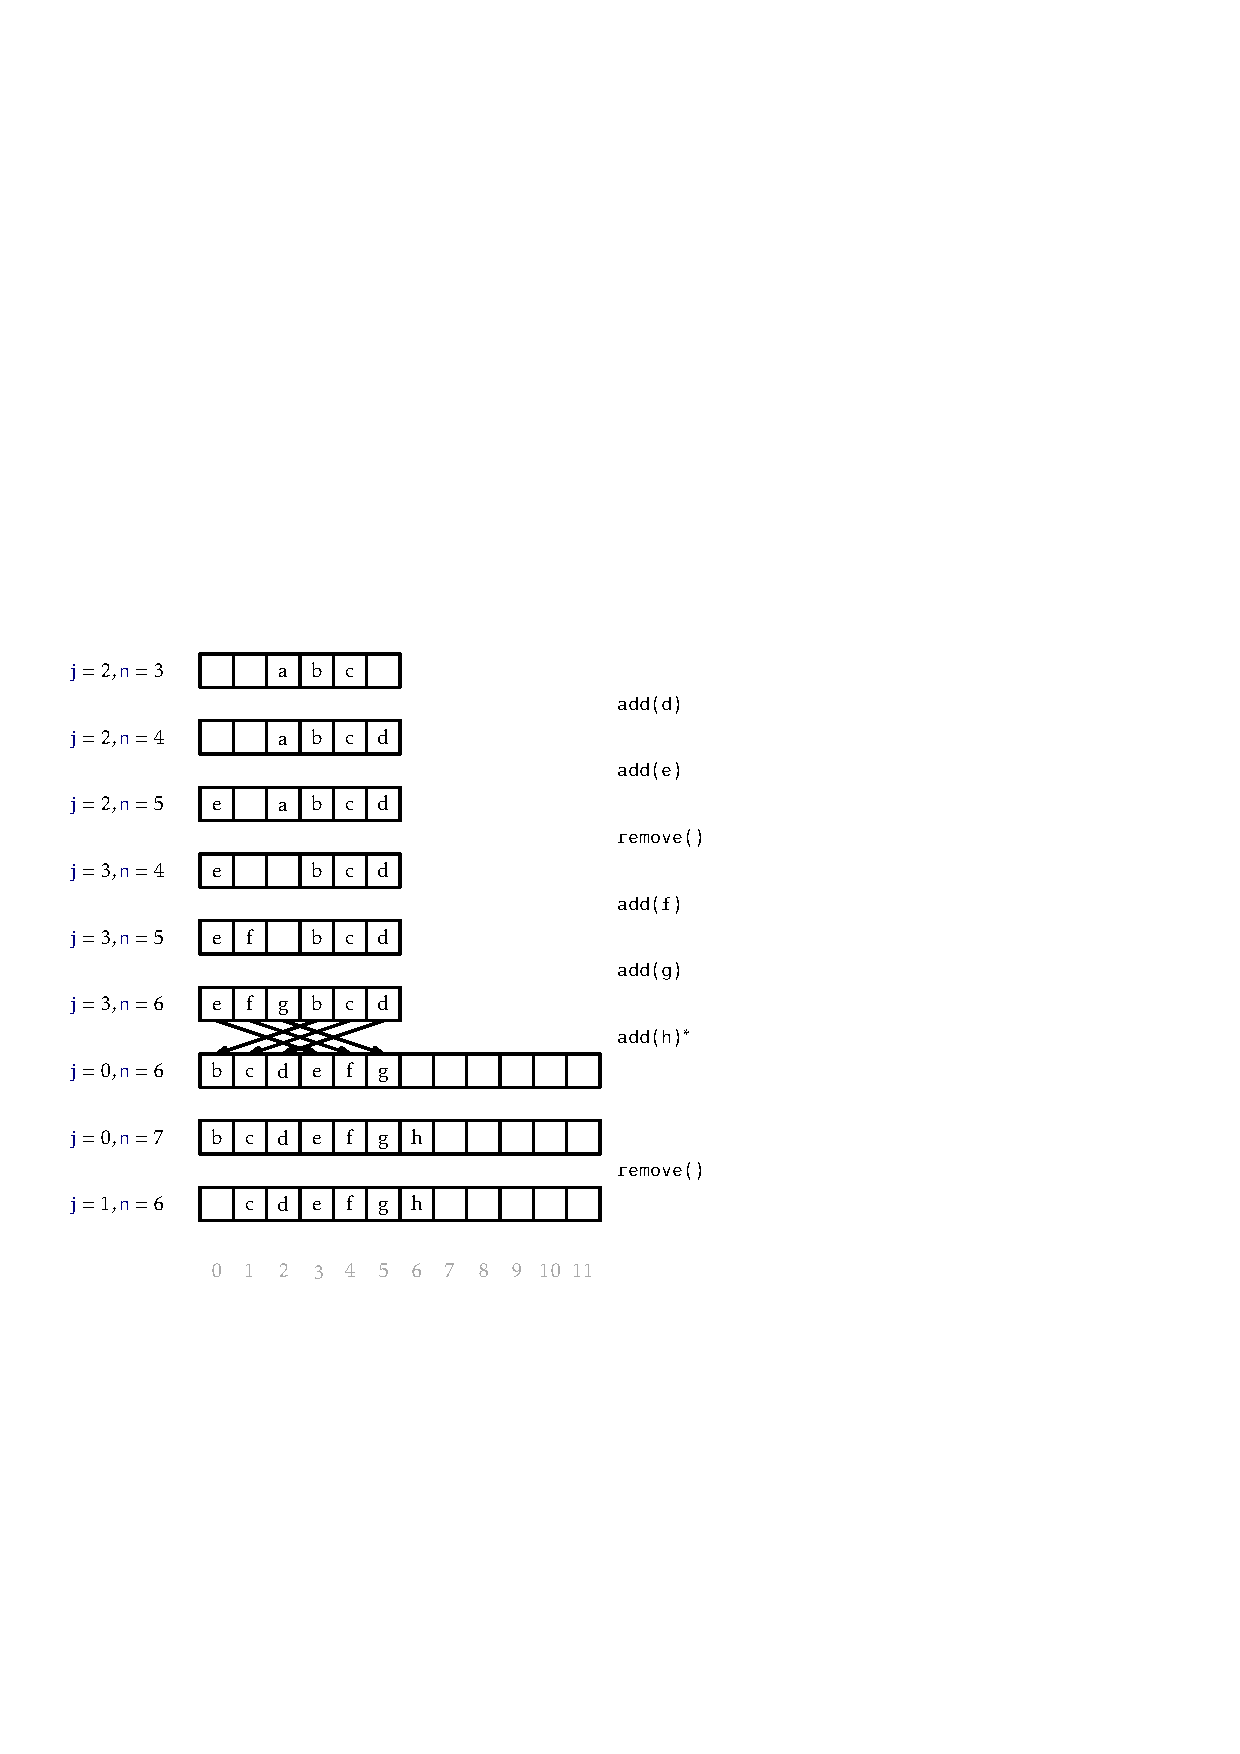
\includegraphics[scale=0.90909]{figs/arrayqueue}
  \end{center}
  \caption[Adicionando e removendo de um ArrayQueue]{Sequência de operações #add(x)# e #remove(i)# em uma
  #ArrayQueue#.  As setas indicam elementos que estão sendo copiados.  Operações que
  resultam em uma chamada de #resize()# estão marcadas com um asterisco.}
  \figlabel{arrayqueue}
\end{figure}



\codeimport{ods/ArrayQueue.add(x)}

Para implementar #remove()#, primeiro armazenamos #a[j]# para que possamos devolvê-lo
mais tarde.  Finalmente, decrementamos #n# e incrementamos #j# (modulo #a.length#)
pela configuração $#j#=(#j#+1)\bmod #a.length#$.  Finalmente, retornamos o valor
armazenado de #a[j]#. Se necessário, podemos chamar #resize()# para diminuir o
tamanho de #a#.

\codeimport{ods/ArrayQueue.remove()}

Finalmente, a operação #resize()# é muito similar à operação #resize()#
de #ArrayStack#.  Aloca um novo array, #b#, de tamanho $2#n#$
e copia
\[
   #a[j]#,#a[(j+1)%a.length]#,\ldots,#a[(j+n-1)%a.length]#
\]
para
\[
   #b[0]#,#b[1]#,\ldots,#b[n-1]#
\]
e faz $#j#=0$.

\codeimport{ods/ArrayQueue.resize()}

\subsection{Resumo}

O seguinte teorema resume o desempenho da estrutura de dados
#ArrayQueue#:

\begin{thm}
Um #ArrayQueue# implementa a interface de #Fila# (FIFO).  Ignorando o custo de
chamada para #resize()#, um #ArrayQueue# suporta as operações
#add(x)# e #remove()# com tempo por operação de $O(1)$.
Além disso, começando com um #ArrayQueue# vazio, qualquer sequência de $m$
operações #add(i,x)# e #remove(i)#  resultam em um tempo gasto total de $O(m)$
 durante todas as chamadas para #resize()#.
\end{thm}

%TODO: Discuss the use of bitwise-and as a replacement for the mod operator

\section{#ArrayDeque#: Operações Rápidas em um Deque Usando um Array}
\seclabel{arraydeque}

\index{ArrayDeque@#ArrayDeque#}%
Um #ArrayQueue# da seção anterior é uma estrutura de dados para
representar uma sequência que nos permite adicionar eficientemente a um
extremidade da sequência e remover da outra extremidade.  A estrutura
de dados #ArrayDeque# permite uma adição e remoção eficientes em ambas as extremidades.
Essa estrutura implementa a interface #Lista# usando a mesma técnica de array
circular usada para representar um #ArrayQueue#.

\codeimport{ods/ArrayDeque.a.j.n}

As operações #get(i)# e #set(i,x)# em um #ArrayDeque# são
diretas.  Elas obtêm ou definem o elemento do array $#a[#{#(j+i)#\bmod
#a.length#}#]#$.

\codeimport{ods/ArrayDeque.get(i).set(i,x)}

A implementação de #add(i,x)# é um pouco mais interessante.  Como
de costume, primeiro verifica se #a# está cheio e, se necessário, chama
#resize()# para redimensionar #a#.  Lembre-se que queremos que esta operação seja
rápida quando #i# é pequeno (perto de 0) ou quando #i# é grande (perto de
#n#).  Portanto, verificamos se $#i#<#n#/2$.  Se sim, deslocamos os
elementos $#a[0]#,\ldots,#a[i-1]#$ para a esquerda.  Caso contrário
($#i#\ge#n#/2$), deslocamos os elementos $#a[i]#,\ldots,#a[n-1]#$ para a
direita. Veja \figref{arraydeque} para uma ilustração das
operações #add(i,x)# e #remove(x)# em um #ArrayDeque#.

%Fim Ester

\begin{figure}
  \begin{center}
    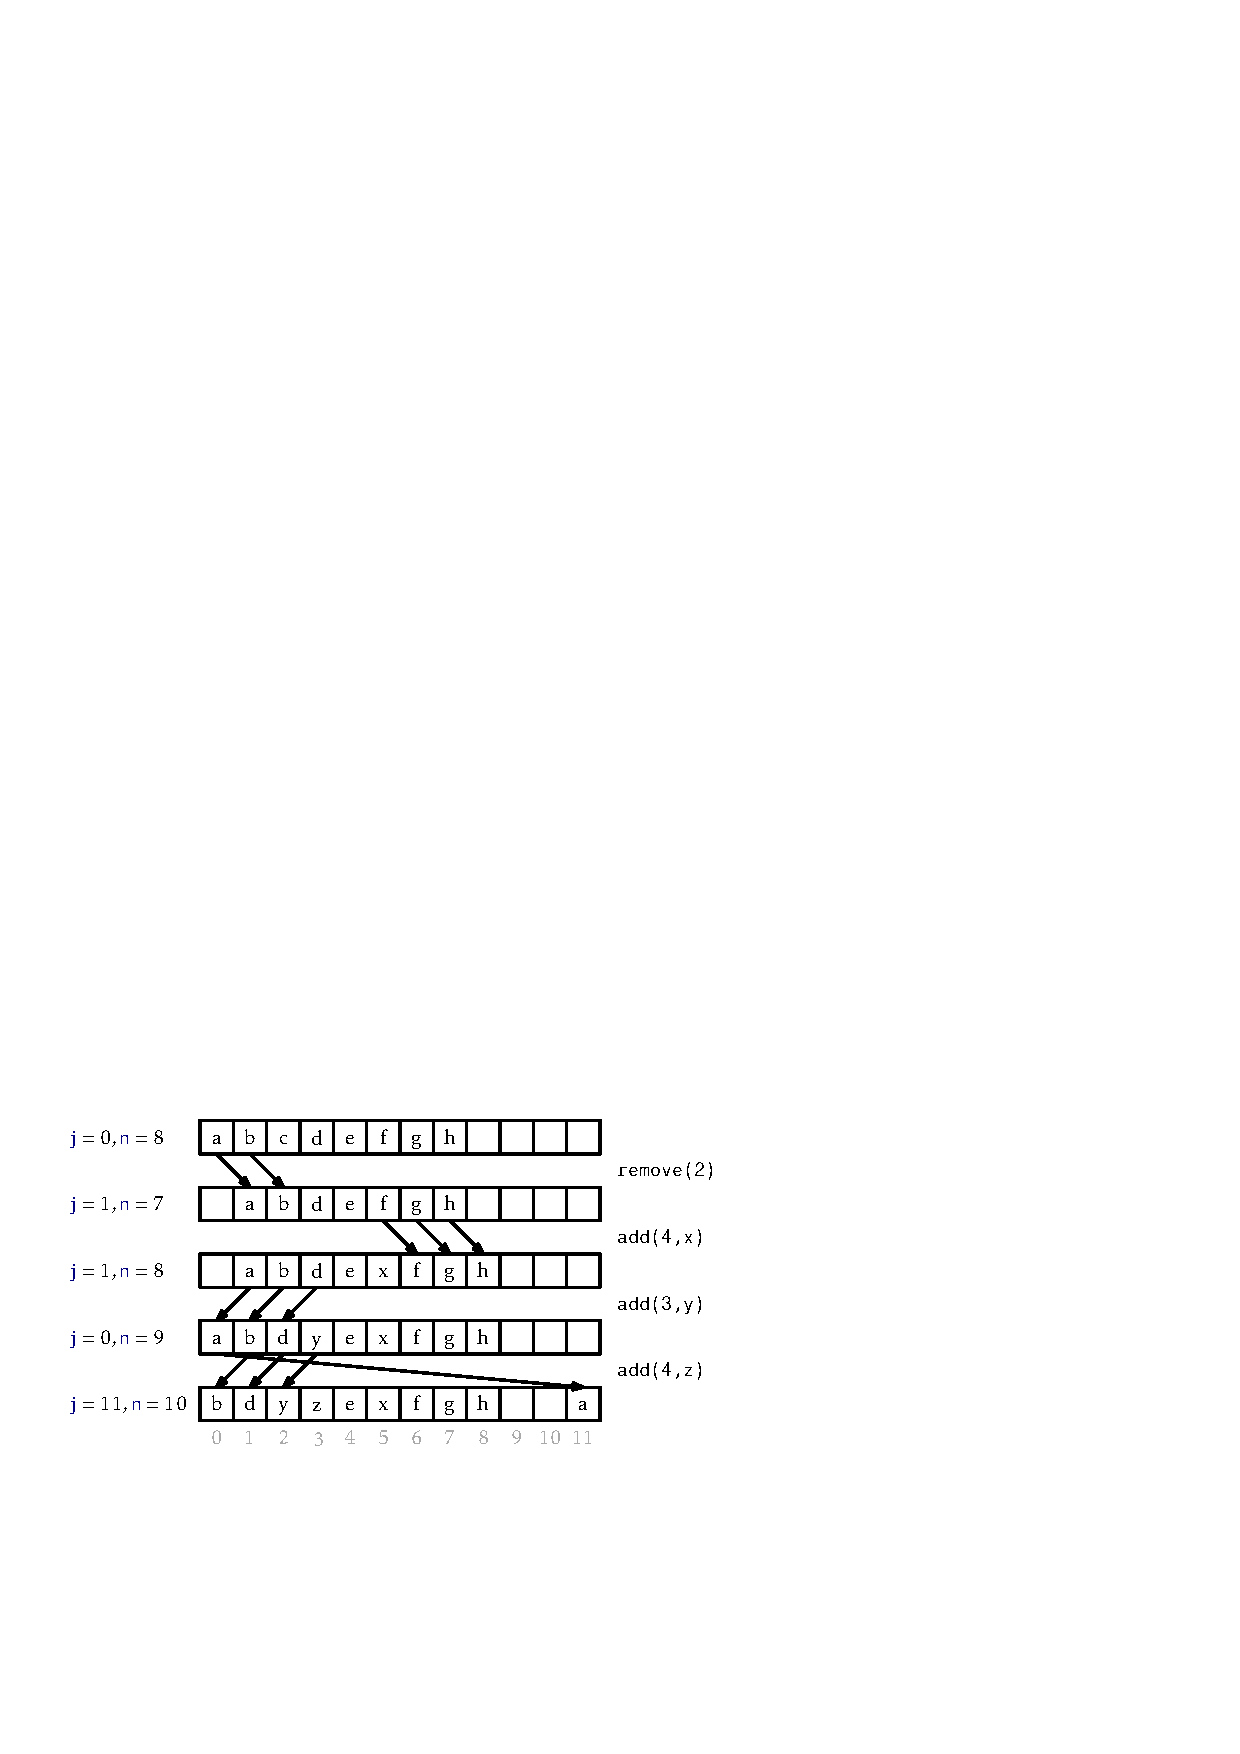
\includegraphics[scale=0.90909]{figs/arraydeque}
  \end{center}
  \caption[Adicionando e removendo de um ArrayDeque]{Uma sequência de operações 
  #add(i,x)# e #remove(i)# em um #ArrayDeque#. As setas indicam elementos que 
  estão sendo copiados.}
  \figlabel{arraydeque}
\end{figure}


\codeimport{ods/ArrayDeque.add(i,x)}

Ao fazer o deslocamento desta maneira, garantimos que #add(i,x)# nunca 
tenha que deslocar mais de $\min\{ #i#, #n#-#i# \}$ elementos. Assim, o 
tempo de execução da operação #add(i,x)# (ignorando o custo de uma operação 
#resize()#) é $O(1+\min\{#i#,#n#-#i#\})$.

A implementação da operação #remove(i)# é semelhante. Desloca os elementos 
$#a[0]#,\ldots,#a[i-1]#$ à direita por uma posição ou desloca os elementos 
$#a[i+1]#,\ldots,#a[n-1]#$ para esquerda por uma posição dependendo se 
$#i#<#n#/2$. Novamente, isso significa que #remove(i)# nunca gasta mais do 
que um tempo $O(1+\min\{#i#,#n#-#i#\})$ para deslocar elementos.

\codeimport{ods/ArrayDeque.remove(i)}

\subsection{Resumo}

O seguinte teorema resume o desempenho da estrutura de dados 
#ArrayDeque#:
\begin{thm}\thmlabel{arraydeque}
  Um #ArrayDeque# implementa a interface #Lista#. Ignorando o custo das chamadas para 
  #resize()#, um #ArrayDeque# suporta as operações
  \begin{itemize}
    \item #get(i)# e #set(i,x)# com tempo de $O(1)$ por operação; e
    \item #add(i,x)# e #remove(i)# com tempo $O(1+\min\{#i#,#n#-#i#\})$  por operação.
  \end{itemize}
  Além disso, começando com um #ArrayDeque# vazio, executar qualquer sequência de $m$ 
  operações #add(i,x)# e #remove(i)# resulta em um total de $O(m)$ de tempo gasto 
  durante todas as chamadas para #resize()#.
\end{thm}

\section{#DualArrayDeque#: Construindo um Deque com Duas Pilhas}
\seclabel{dualarraydeque}

\index{DualArrayDeque@#DualArrayDeque#}%
Em seguida, apresentamos uma estrutura de dados, o #DualArrayDeque# 
que atinge os mesmos limites de desempenho que um #ArrayDeque# usando 
dois #ArrayStack#s. Embora o desempenho assintótico do #DualArrayDeque# 
não seja melhor do que o #ArrayDeque#, ainda vale a pena estudar, 
uma vez que oferece um bom exemplo de como fazer uma estrutura de dados 
sofisticada, combinando duas estruturas de dados mais simples.

O #DualArrayDeque# representa uma lista usando dois #ArrayStack#s. 
Lembre-se de que #ArrayStack# é rápido quando as operações nele 
modificam elementos perto do final. O #DualArrayDeque# coloca dois 
#ArrayStack#s, chamados de #front# e #back#, unidos pelos suas extremidades, 
para que as operações sejam rápidas em qualquer extremidade.

\codeimport{ods/DualArrayDeque.front.back}

O #DualArrayDeque# não armazena explicitamente o número, #n#, 
de elementos que ele contém. Ele não precisa, uma vez que contém 
$#n#=#front.size()# + #back.size()#$ elementos. No entanto, ao 
analisar o #DualArrayDeque# vamos ainda usar #n# para indicar 
o número de elementos que ele contém.

\codeimport{ods/DualArrayDeque.size()}

O #front# do #ArrayStack# armazena os elementos da lista cujos índices 
são $0,\ldots,#front.size()#-1$, mas os armazena na ordem inversa. O #back# do 
#ArrayStack# contém elementos da lista com índices em $#front.size()#,\ldots,#size()#-1$ 
na ordem normal. Desta forma, #get(i)# e #set(i, x)# traduzem para chamadas 
apropriadas para #get(i)# ou #set(i,x)# em #front# ou #back#, levando um tempo de 
$O(1)$ por operação.

\codeimport{ods/DualArrayDeque.get(i).set(i,x)}

Note que se um índice $#i#<#front.size()#$, então ele corresponde ao elemento 
de #front# na posição $#front.size()#-#i#-1$, uma vez que os elementos de 
#front# são armazenados na ordem inversa.

Adicionar e remover elementos de um #DualArrayDeque# é ilustrado na 
\figref{dualarraydeque}. A operação #add(i,x)# manipula ou #front# ou #back#, 
conforme apropriado:

\begin{figure}
  \begin{center}
    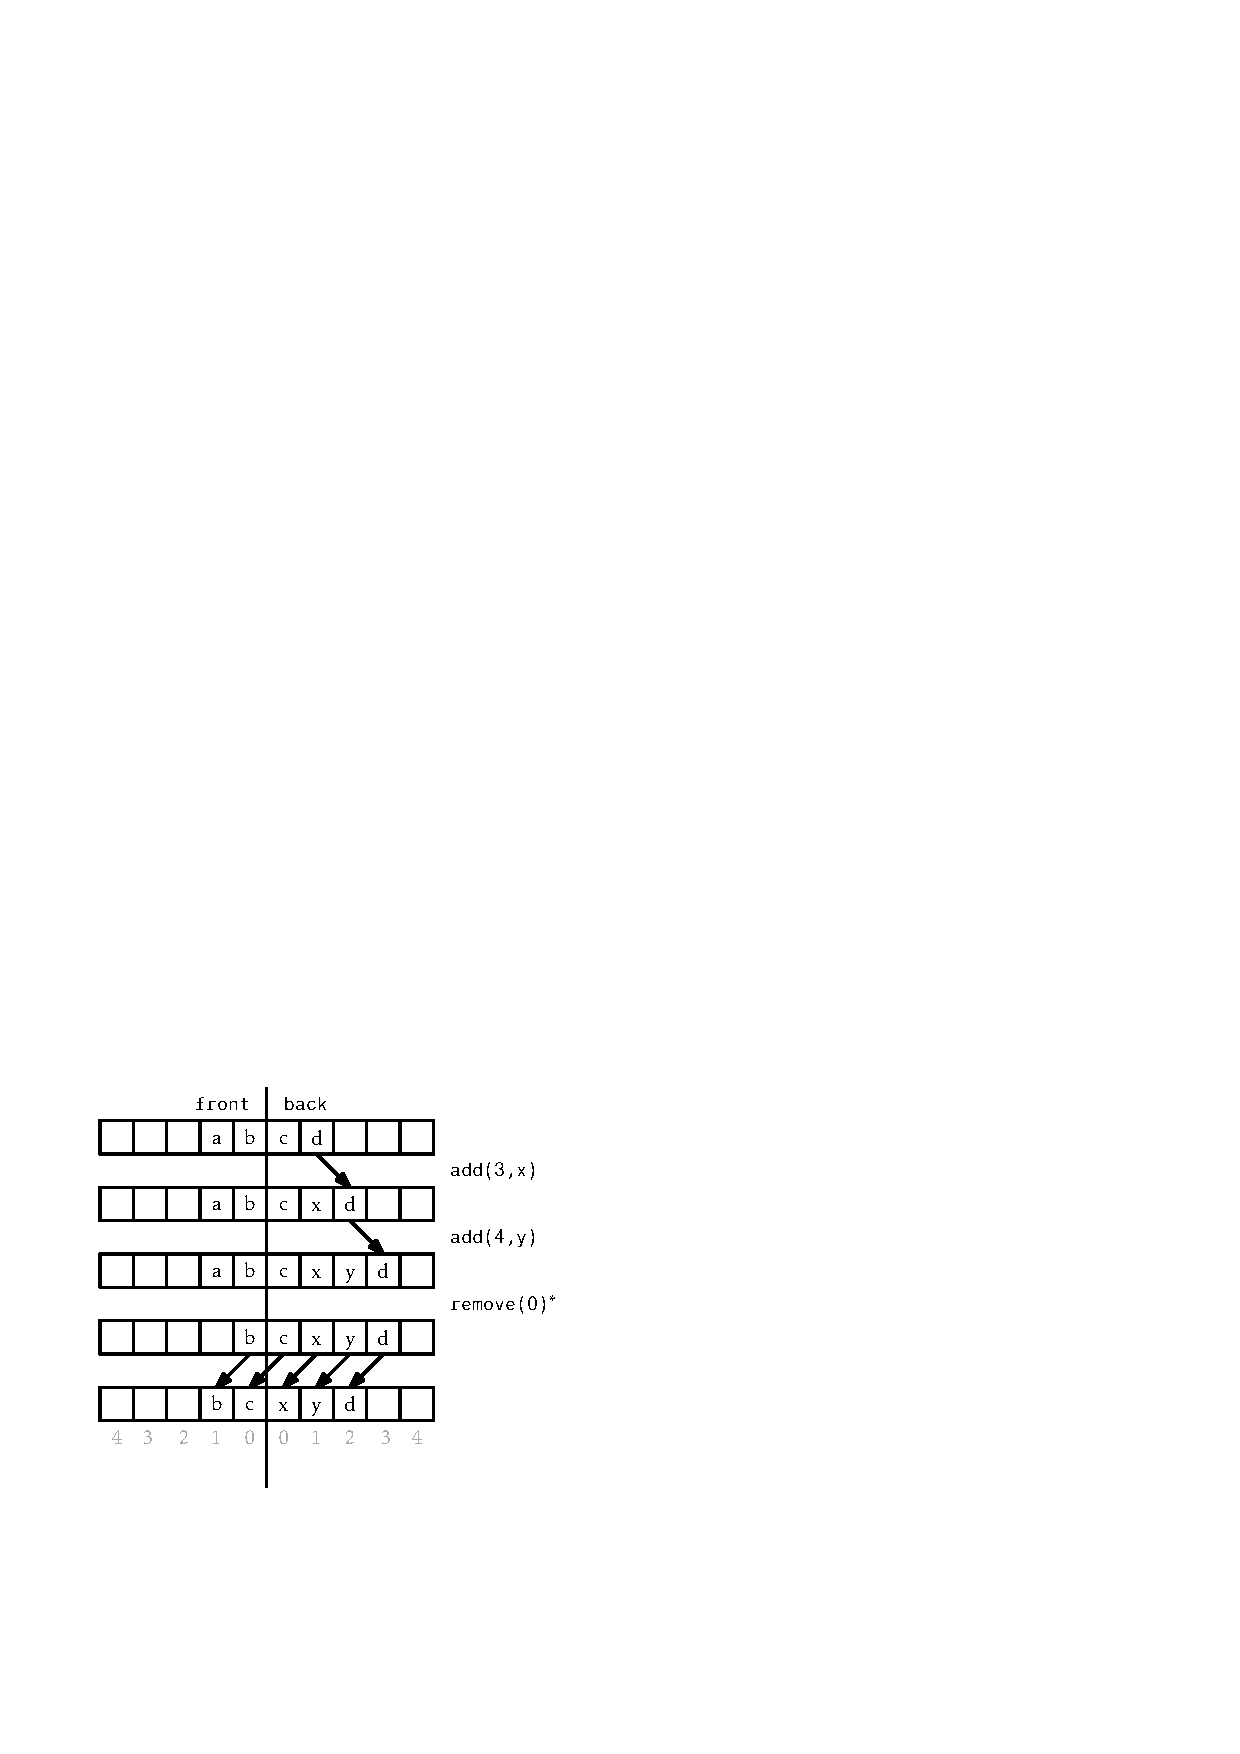
\includegraphics[scale=0.90909]{figs/dualarraydeque}
  \end{center}
  \caption[Adicionando e removendo em um DualArrayDeque]{Uma sequência de operações 
  #add(i, x)# e #remove(i)# em um #DualArrayDeque#. As setas indicam elementos 
  que estão sendo copiados. Operações que resultam em um rebalanceamento por 
  #balance()# são marcadas com um asterisco.}
  \figlabel{dualarraydeque}
\end{figure}



\codeimport{ods/DualArrayDeque.add(i,x)}

O método #add(i,x)# realiza o reequilíbrio dos dois #ArrayStack#s #front# e 
#back#, chamando o método #balance()#. A implementação de #balance()# é descrita 
abaixo, mas por agora é suficiente saber que #balance()# garante que, a menos 
que $#size()#<2$, #front.size()# e #back.size()# não diferem em mais de um 
fator de 3. Em particular, $3\cdot#front.size()# \ge #back.size()#$ e
$3\cdot#back.size()# \ge #front.size()#$.

Em seguida, analisamos o custo de #add(i,x)#, ignorando o custo das chamadas 
para #balance()#. Se $#i#<#front.size()#$, então #add(i,x)# é implementada 
pela chamada para $#front.add(front.size()-i-1,x)#$. Posto que #front# é 
um #ArrayStack#, o custo desta é
\begin{equation}
  O(#front.size()#-(#front.size()#-#i#-1)+1) = O(#i#+1) \enspace .
  \eqlabel{das-front}
\end{equation}
Por outro lado, se $#i#\ge#front.size()#$, então #add(i,x)# é 
implementado como $#back.add(i-front.size(),x)#$. O custo disso é
\begin{equation}
  O(#back.size()#-(#i#-#front.size()#)+1) = O(#n#-#i#+1) \enspace .
  \eqlabel{das-back}
\end{equation}

Observe que o primeiro caso \myeqref{das-front} ocorre quando $#i#<#n#/4$.
O segundo caso \myeqref{das-back} ocorre quando $#i#\ge 3#n#/4$. Quando 
$#n#/4\le#i#<3#n#/4$, não podemos ter certeza se a operação afeta 
#front# ou #back#, mas em ambos os casos, a operação leva um tempo 
$O(#n#)=O(#i#)=O(#n#-#i#)$, uma vez que $#i#\ge #n#/4$ e $#n#-#i#>
#n#/4$. Resumindo a situação, temos
\[
     \mbox{Tempo de execução de } #add(i,x)# \le 
          \begin{cases}
            O(1+ #i#) & \mbox{se $#i#< #n#/4$} \\
            O(#n#) & \mbox{se $#n#/4 \le #i# < 3#n#/4$} \\
            O(1+#n#-#i#) & \mbox{se $#i# \ge 3#n#/4$}
          \end{cases}.
\]
Assim, o tempo de execução de #add(i,x)#, se ignorarmos o custo da chamada 
para #balance()#, é $O(1+\min\{#i#, #n#-#i#\})$.

%Lucas
A operação #remove(i)# e sua análise se assemelham à operação e 
análise de #add(i,x)#.

\codeimport{ods/DualArrayDeque.remove(i)}

\subsection{Balanceamento}

Finalmente, voltamos para a operação #balance()# executada por #add(i,x)# 
e #remove(i)#. Esta operação garante que nem #front# nem #back# tornem-se 
muito grandes (ou muito pequenos). Garante que, a menos que haja menos de 
dois elementos, #front# e #back# contenham, cada um, pelo menos $#n#/4$
elementos. Se este não for o caso, então ela move elementos entre eles
de modo que #front# e #back# contenham exatamente $\lfloor#n#/2\rfloor$ 
elementos e $\lceil#n#/2\rceil$ elementos, respectivamente.

\codeimport{ods/DualArrayDeque.balance()}

Aqui há pouco para analisar. Se #balance()# faz o rebalanceamento, então 
ela move $O(#n#)$ elementos e isso leva um tempo $O(#n#)$. Isso é ruim 
uma vez que #balance()# é chamada juntamente com cada chamada de 
#add(i,x)# e #remove(i)#. Porém, o seguinte lema mostra que, em média, 
#balance()# só gasta uma quantidade constante de tempo por operação.

\begin{lem}\lemlabel{dualarraydeque-amortized}
	Se um #DualArrayDeque# vazio for criado, e qualquer sequência de $m\ge 1$
	chamadas de #add(i,x)# e #remove(i)# ocorrerem, então o tempo total gasto 
	durante todas as chamadas de #balance()# é $O(m)$.
\end{lem}

\begin{proof}
	Vamos mostrar que se #balance()# é forçada a deslocar elementos, então,
	o número de operações #add(i,x)# e #remove(i)# desde a última vez que 
	quaisquer elementos foram deslocados por #balance()# é pelo menos 
	$#n#/2-1$. Como na prova do \lemref{arraystack-amortized}, isso é 
	suficiente para provar que o tempo total gasto por #balance()# é $O(m)$.
	
	Realizaremos nossa análise utilizando uma técnica conhecida como
	\emph{método potencial}.
	\index{potential}%
	\index{potential method}%
	Defina o \emph{potencial}, $\Phi$, do
	#DualArrayDeque# como a diferença de tamanho entre #front# e #back#:
	\[  \Phi = |#front.size()# - #back.size()#| \enspace . \]
	O interessante sobre este potencial é que uma chamada de #add(i,x)#
	ou #remove(i)# que não faz nenhum balanceamento pode aumentar o 
	potencial por no máximo 1.
	
	Observe que, imediatamente após uma chamada a #balance()# que desloque
	elementos, o potencial, $\Phi_0$, é pelo menos 1, posto que
	\[ \Phi_0 = \left|\lfloor#n#/2\rfloor-\lceil#n#/2\rceil\right|\le 1  \enspace .\]
	
	Considere a situação imediatamente antes de uma chamada #balance()# que
	desloca elementos, e suponha, sem perda de generalidade, que #balance()#
	está deslocando elementos porque $3#front.size()# < #back.size()#$.
	Observe que, neste caso,
	\begin{eqnarray*}
		#n# & = & #front.size()#+#back.size()# \\
		& < & #back.size()#/3+#back.size()# \\
		& = & \frac{4}{3}#back.size()#
	\end{eqnarray*}
	Além disso, o potencial neste momento é
	\begin{eqnarray*}
		\Phi_1 & = & #back.size()# - #front.size()# \\
		&>& #back.size()# - #back.size()#/3 \\
		&=& \frac{2}{3}#back.size()# \\
		&>& \frac{2}{3}\times\frac{3}{4}#n# \\
		&=& #n#/2
	\end{eqnarray*}
	Portanto, o número de chamadas #add(i,x)# ou #remove(i)# desde a última
	vez que #balance()# deslocou elementos é pelo menos $\Phi_1-\Phi_0
	> #n#/2-1$. Isso completa a prova.
\end{proof}

\subsection{Resumo}

O seguinte teorema resume as propriedades de um #DualArrayDeque#:

\begin{thm}\thmlabel{dualarraydeque}
	O #DualArrayDeque# implementa a interface #Lista#. Ignorando o
	custo de chamadas #resize()# e #balance()#, um #DualArrayDeque#
	suporta as operações
	\begin{itemize}
		\item #get(i)# e #set(i,x)# com um tempo $O(1)$ por operação; e
		\item #add(i,x)# e #remove(i)# com um tempo $O(1+\min\{#i#,#n#-#i#\})$ 
		por operação.
	\end{itemize}
	Além disso, começando com um #DualArrayDeque# vazio, qualquer sequência
	de $m$ operações #add(i,x)# e #remove(i)# resulta em um tempo total gasto
	de $O(m)$ durante todas as chamadas a #resize()# e #balance()#.
\end{thm}


\section{#RootishArrayStack#: Um Array Stack Eficiente em Espaço}
\seclabel{rootisharraystack}

\index{RootishArrayStack@#RootishArrayStack#}%
Uma das desvantagens de todas as estruturas de dados anteriores neste 
capítulo é que, porque armazenam seus dados em um ou dois arrays e evitam
o redimensionamento desses arrays com muita frequência, os arrays 
frequentemente não estão muito cheios. Por exemplo, imediatamente após uma
operação #resize()# em um #ArrayStack#, o array de base #a# está apenas 
meio cheio. Pior ainda, há momentos no qual apenas um terço de #a# contém dados.

Nesta seção, discutimos a estrutura de dados #RootishArrayStack#,
que aborda o problema do desperdício de espaço. O #RootishArrayStack#
armazena #n# elementos usando $O(\sqrt{#n#})$ arrays. Nesses arrays, no
máximo $O(\sqrt{#n#})$ locais do array ficam sem utilização. Todos
os locais restantes são usados para armazenar dados. Portanto, essas
estruturas de dados desperdiçam um espaço de no máximo $O(\sqrt{#n#})$ 
ao armazenar #n# elementos.

Uma #RootishArrayStack# armazena seus elementos em uma lista de #r#
arrays chamados \emph{blocos}, que são numerados $0,1,\ldots,#r#-1$.
Veja \figref{rootisharraystack}. O bloco $b$ contém $b+1$ elementos.
Portanto, todos os blocos #r# contêm um total de
\[
1+ 2+ 3+\cdots +#r# = #r#(#r#+1)/2
\]
elementos. A fórmula acima pode ser obtida como mostrado na \figref{gauss}.

\begin{figure}
	\begin{center}
		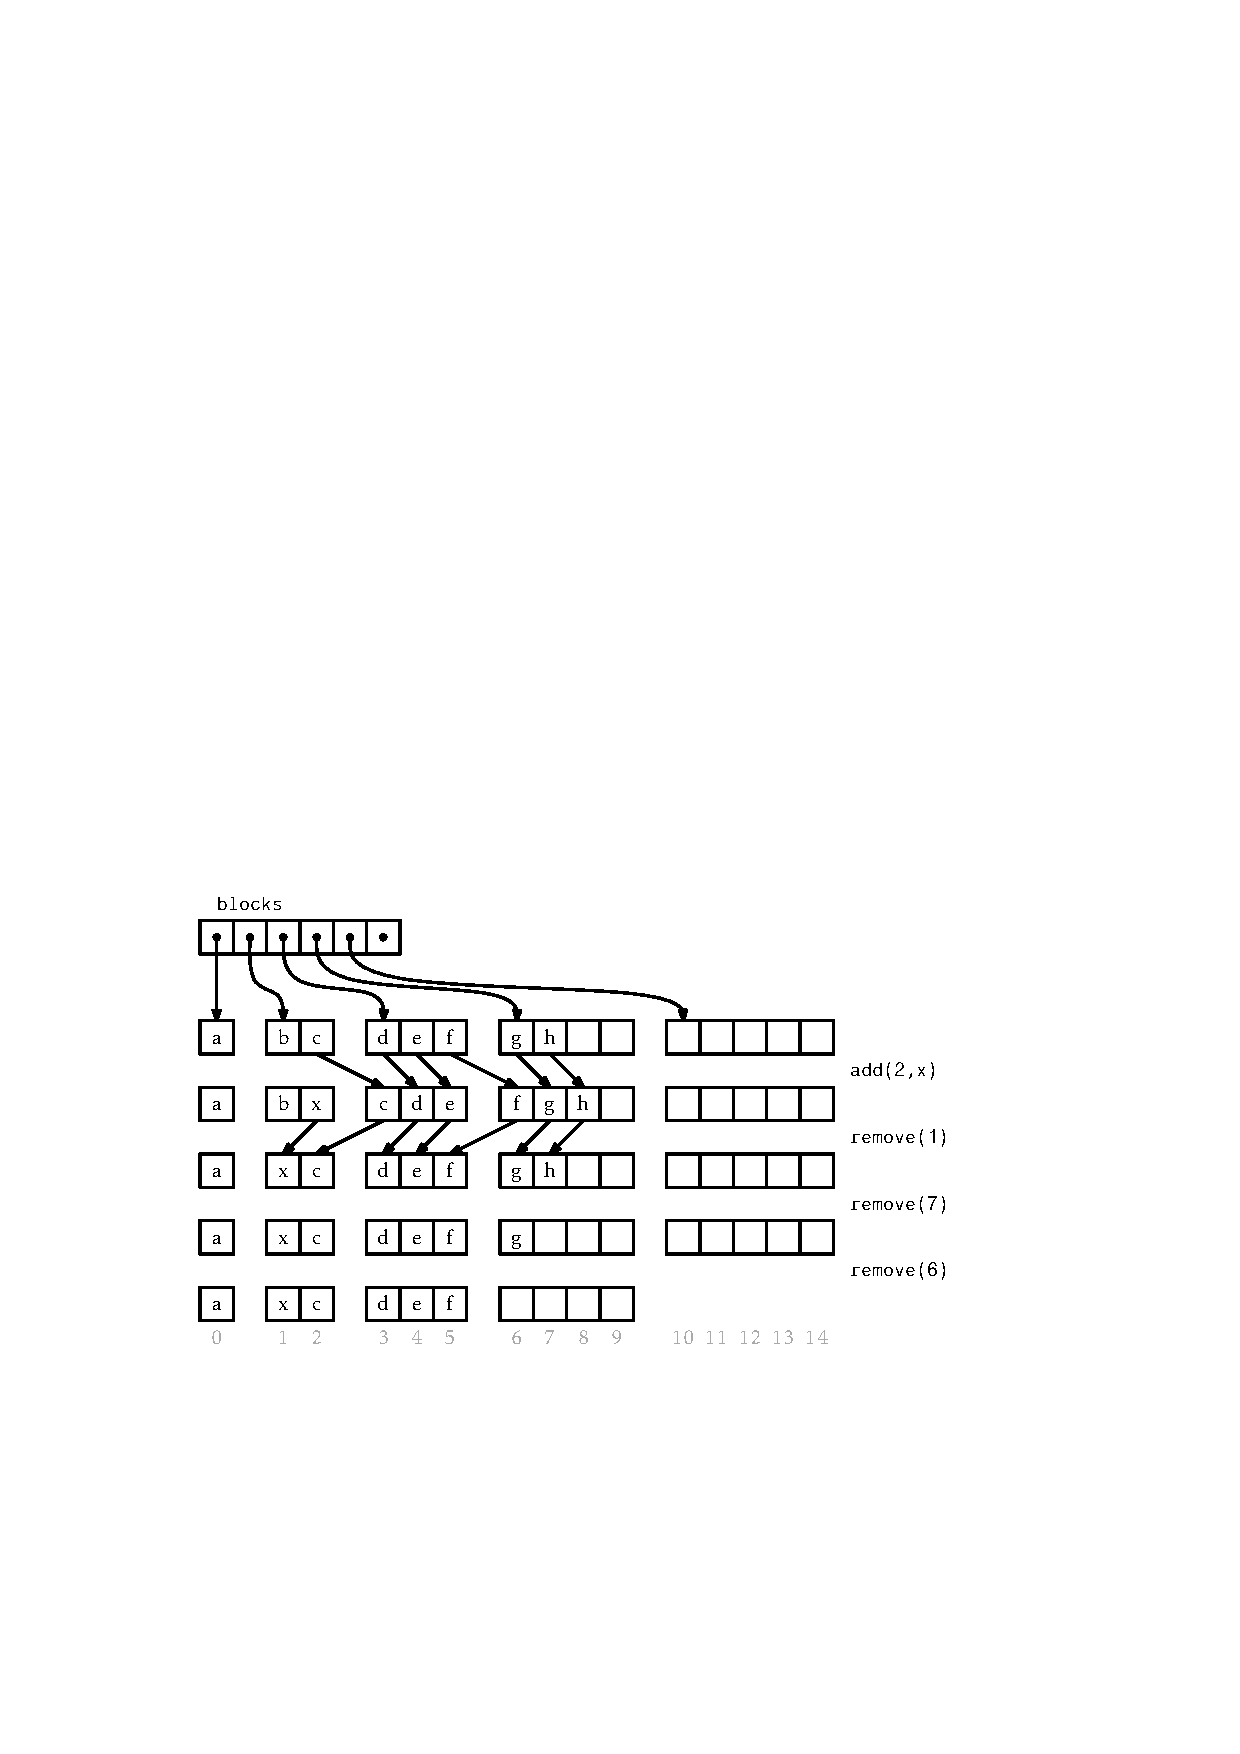
\includegraphics[width=\ScaleIfNeeded]{figs/rootisharraystack}
	\end{center}
	\caption[Adicionando ou removendo em um RootishArrayStack]{Uma sequência de operações #add(i,x)# e #remove(i)# em um
		#RootishArrayStack#.  As flechas indicam elementos sendo copiados. }
	\figlabel{rootisharraystack}
\end{figure}

\codeimport{ods/RootishArrayStack.blocks.n}

\begin{figure}
  \begin{center}
    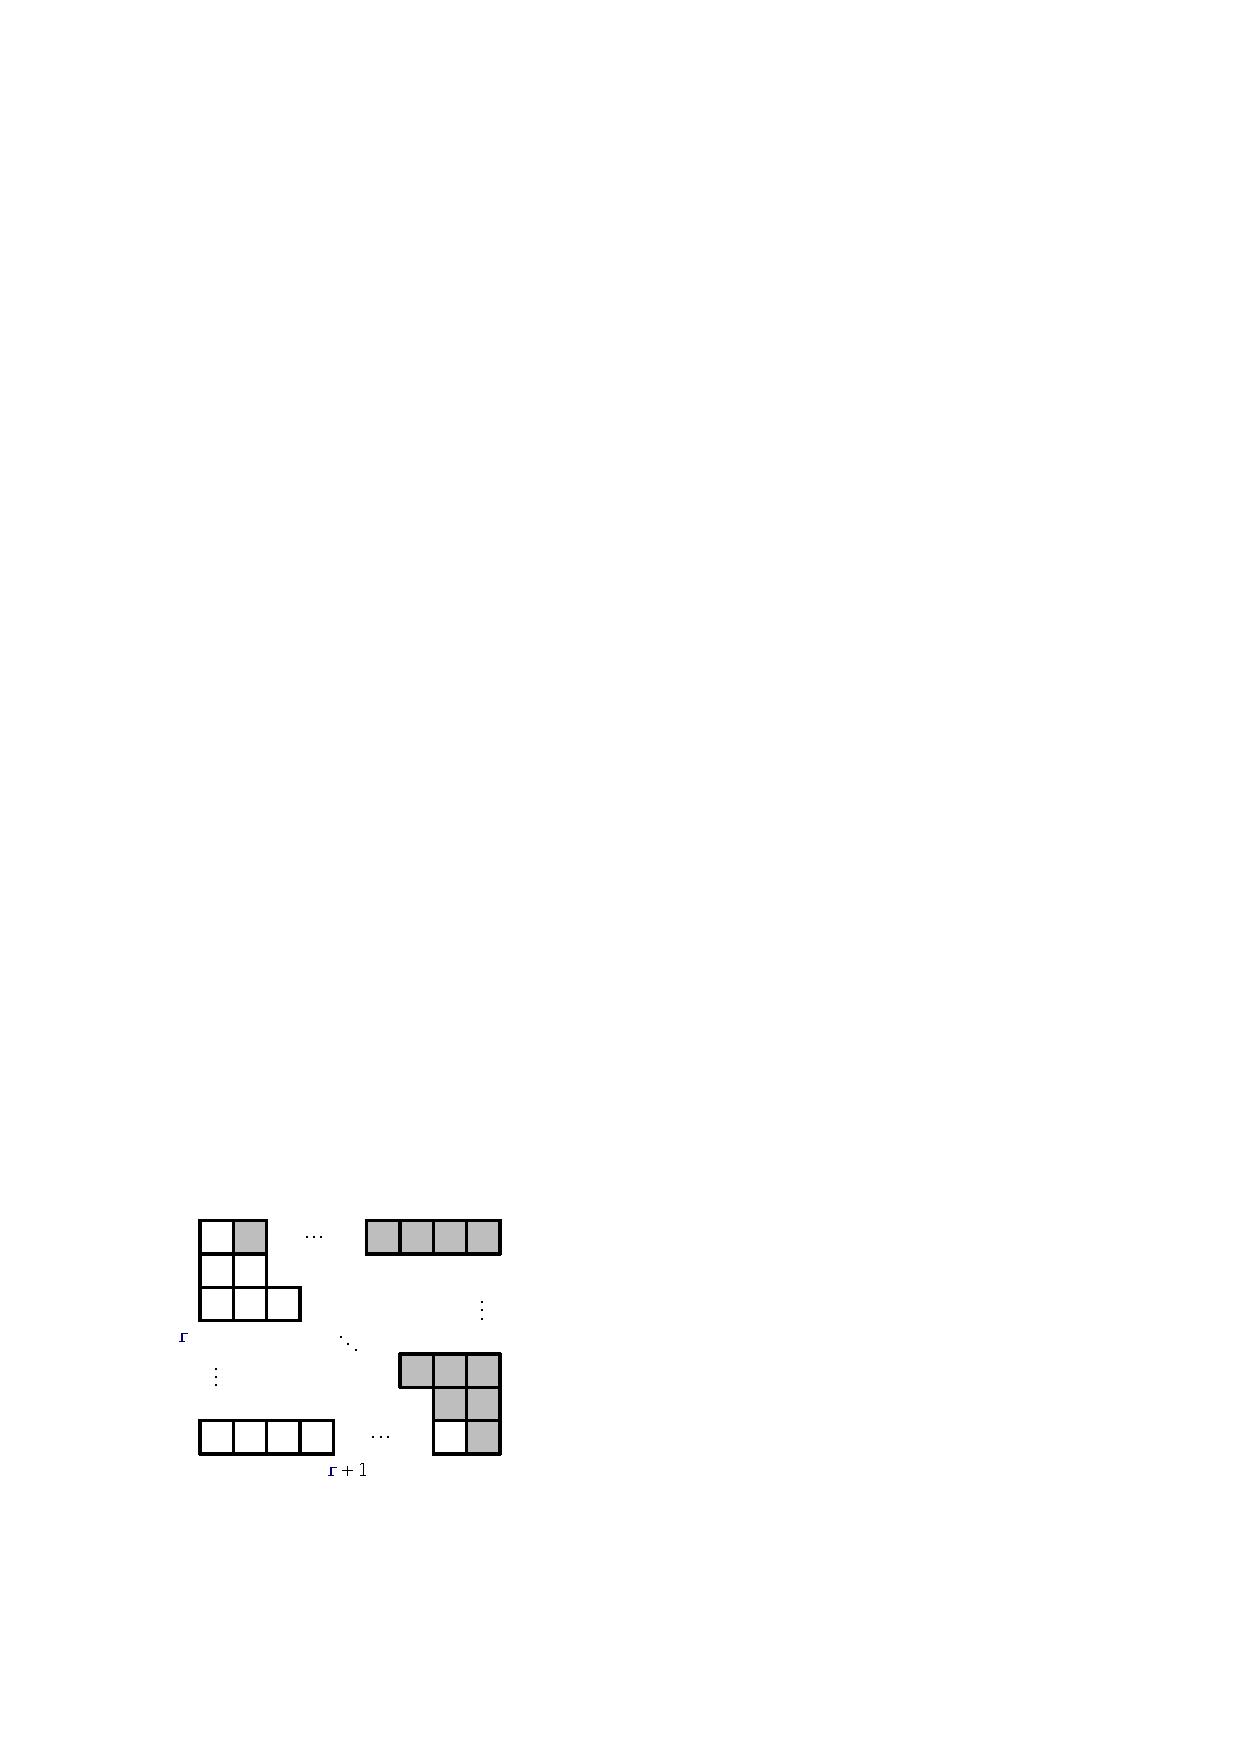
\includegraphics[scale=0.90909]{figs/gauss}
  \end{center}
  \caption{O número de quadrados brancos é $1+2+3+\cdots+#r#$.  O número de
  quadrados cinzas é o mesmo.  Juntando os quadrados brancos e cinzas cria
  um retângulo consistindo de $#r#(#r#+1)$ quadrados.}
  \figlabel{gauss}
\end{figure}
%Fim Lucas

%Matheus
Como seria de esperar, os elementos da lista são dispostos dentro dos blocos.
O elemento de lista com índice 0 é armazenado no bloco 0, os elementos com índices 
de lista 1 e 2 são armazenados no bloco 1, os elementos com índices de lista 3, 
4 e 5 são armazenados no bloco 2 e assim por diante. 
O principal problema que temos de resolver é o de determinar, dado um índice $#i#$,
qual bloco contém #i# bem como o índice correspondente ao #i#
dentro desse bloco.

Determinar o índice de #i# dentro de seu bloco, acaba sendo fácil. Se o
índice #i# está no bloco #b#, então o número de elementos nos blocos
$0,\ldots,#b#-1$ é $#b#(#b#+1)/2$.  Assim sendo, #i# é armazenado no local
\[
#j# = #i# - #b#(#b#+1)/2
\]
dentro do bloco #b#.  
Um pouco mais desafiador é o problema de determinar
o valor de #b#.  O número de elementos com índices inferiores ou iguais 
a #i# é $#i#+1$.  Por outro lado, o número de elementos nos blocos
$0,\ldots,b$ é $(#b#+1)(#b#+2)/2$.  Assim sendo, #b# é o menor
inteiro de tal modo que
\[
(#b#+1)(#b#+2)/2 \ge #i#+1 \enspace .
\]
Podemos reescrever essa equação como
\[
#b#^2 + 3#b# - 2#i# \ge  0 \enspace .
\]
A equação quadrática correspondente $#b#^2 + 3#b# - 2#i# =  0$ possui duas
soluções: $#b#=(-3 + \sqrt{9+8#i#}) / 2$ e $#b#=(-3 - \sqrt{9+8#i#}) / 2$.
A segunda solução não faz sentido em nossa aplicação, 
pois ela sempre dá um valor negativo. Assim sendo, obtemos a solução $#b# = (-3 +
\sqrt{9+8i}) / 2$.  Em geral, essa solução não é um inteiro, mas voltando à nossa desigualdade, 
queremos o menor número inteiro $#b#$ de tal modo que 
$#b# \ge (-3 + \sqrt{9+8i}) / 2$.  Isto é simplesmente
\[
#b# = \left\lceil(-3 + \sqrt{9+8i}) / 2\right\rceil \enspace .
\]

\codeimport{ods/RootishArrayStack.i2b(i)}

Com isso resolvido, os métodos #get(i)# e #set(i,x)# são mais fáceis. 
Primeiro, calculamos o bloco apropriado #b# e o índice apropriado #j# 
dentro do bloco e executamos a operação apropriada:

\codeimport{ods/RootishArrayStack.get(i).set(i,x)}

Se usarmos qualquer estrutura de dados deste capítulo para representar a lista
de #blocos#, então #get(i)# e #set(i,x)# funcionarão em tempo constante.

O método #add(i,x)# será, agora, familiar.  
Verificamos primeiro se a nossa estrutura de dados está cheia, 
verificando se o número de blocos, #r#, é tal que $#r#(#r#+1)/2 = #n#$. 
Se sim, chamamos #grow()#
para adicionar outro bloco.  Feito isso, deslocamos elementos com índices
$#i#,\ldots,#n#-1$ para a direita de uma posição para dar espaço para o
novo elemento com índice #i#:

\codeimport{ods/RootishArrayStack.add(i,x)}

O método #grow()# faz o que esperamos. Adiciona um novo bloco:

\codeimport{ods/RootishArrayStack.grow()}

Ignorando o custo da operação #grow()#, o custo da operação #add(i,x)# 
é dominado pelo custo da mudança e é portanto
$O(1+#n#-#i#)$, exatamente como um #ArrayStack#.

A operação #remove(i)# é similar a #add(i,x)#.  Desloca 
os elementos com índices $#i#+1,\ldots,#n#$ uma posição para a esquerda e então,
se tiver mais de um bloco vazio, é chamado o método #shrink()# 
para remover todos exceto um dos blocos não usados:

\codeimport{ods/RootishArrayStack.remove(i)}
\codeimport{ods/RootishArrayStack.shrink()}

Mais uma vez, ignorando o custo da operação #shrink()# , o custo da 
operação #remove(i)# é dominado pelo custo do deslocamento e é
portanto $O(#n#-#i#)$.

\subsection{Análise de Crescimento e Diminuição}

A análise acima de #add(i,x)# e #remove(i)# não representa o custo
de #grow()# e #shrink()#.  Note que, diferentemente da operação
#ArrayStack.resize()# , #grow()# e #shrink()# não copiam
nenhum dado.  Eles apenas alocam ou liberam um array de tamanho #r#.  Em
alguns ambientes, isso leva apenas um tempo constante, enquanto em outros, pode
requerer tempo proporcional a #r#.

Notamos que, imediatamente após chamar #grow()# ou #shrink()#, a
situação é clara. O bloco final está completamente vazio, e todos os outros
blocos estão completamente cheios.  Outra chamada para #grow()# ou #shrink()# não irá acontecer 
até pelo menos $#r#-1$ elementos terem sido adicionados ou removidos.
Assim sendo, mesmo que #grow()# e #shrink()# levem um tempo $O(#r#)$, esse
custo pode ser amortizado por pelo menos $#r#-1$ operações #add(i,x)# ou #remove(i)#, 
de forma que o custo amortizado #grow()# e #shrink()# é
$O(1)$ por operação.

\subsection{Uso de Espaço}
\seclabel{rootishspaceusage}

Em seguida, analisamos a quantidade extra de espaço usado pela #RootishArrayStack#.
Em particular, queremos contar qualquer espaço usado pela #RootishArrayStack# que não seja um elemento do array 
atualmente usado para manter um elemento de lista.  Podemos chamar tal espaço de \emph{espaço desperdiçado}.
\index{wasted space}%

A operação #remove(i)# garante que um #RootishArrayStack# nunca tenha 
mais de dois blocos que não estejam completamente cheios. O número de 
blocos, #r#, usado por #RootishArrayStack# que armazena #n# elementos, 
portanto, satisfaz
\[
    (#r#-2)(#r#-1)/2 \le #n# \enspace .
\]
Novamente, usando a equação quadrática nele fornece
\[
   #r# \le \frac{1}{2}\left(3+\sqrt{8#n#+1}\right) = O(\sqrt{#n#}) \enspace .
\]
Os dois últimos blocos têm tamanhos #r# e #r-1#, então o espaço 
perdido por esses dois blocos é no máximo $2#r#-1 = O(\sqrt{#n#})$. 
Se armazenamos os blocos em (por exemplo) um #ArrayStack#, então a 
quantidade de espaço desperdiçado pela #Lista# que armazena esses 
#r# blocos também é $O(#r#)=O(\sqrt{#n#})$. O outro espaço necessário 
para armazenar #n# e outras informações contábeis é $O(1)$.
Portanto, a quantidade total de espaço desperdiçado em um #RootishArrayStack#
é $O(\sqrt{#n#})$.


Em seguida, argumentamos que este uso do espaço é ideal para qualquer 
estrutura de dados que começa vazia e pode suportar a adição de um item 
de cada vez. Mais precisamente, mostraremos que, em algum ponto durante a 
adição de #n# itens, a estrutura de dados está desperdiçando um espaço de pelo menos $\sqrt{#n#}$ (embora possa estar  
desperdiçado apenas durante um momento).

Suponha que começamos com uma estrutura de dados vazia e adicionamos 
#n# itens, um de cada vez. No final deste processo, todos os #n# itens 
são armazenados na estrutura e distribuídos entre uma coleção de #r# 
blocos de memória. Se $#r#\ge \sqrt{#n#}$, então a estrutura de dados 
deve estar usando #r# ponteiros (ou referências) para acompanhar esses 
#r# blocos, e esses ponteiros são espaço desperdiçado. Por outro lado, 
se $#r# < \sqrt{#n#}$, então, pelo princípio da ``casa de pombos'', algum bloco 
deve ter tamanho de pelo menos $#n#/#r# > \sqrt{#n#}$. Considere o momento 
em que este bloco foi alocado pela primeira vez. Imediatamente após ele 
ter sido alocado, esse bloco estava vazio e, portanto, estava desperdiçando 
$\sqrt{#n#}$ de espaço. Portanto, em algum ponto no tempo durante a inserção 
dos elementos #n#, a estrutura de dados estava desperdiçando $\sqrt{#n#}$ de espaço.

\subsection{Resumo}

O seguinte teorema resume nossa discussão da estrutura de dados #RootishArrayStack#:

\begin{thm}\thmlabel{rootisharraystack}
  Um #RootishArrayStack# implementa a interface #Lista#. Ignorando o custo das chamadas 
  para #grow()# e #shrink()#, um #RootishArrayStack# suporta as operações
  \begin{itemize}
    \item #get(i)# e #set(i,x)# com tempo $O(1)$ por operação; e
    \item #add(i,x)# e #remove(i)# com tempo $O(1+#n#-#i#)$ por operação.
  \end{itemize}
  Além disso, começando com um #RootishArrayStack# vazio, qualquer sequência de $m$ 
  operações #add(i,x)# e #remove(i)# resulta em um tempo gasto total de $O(m)$  
  durante todas as chamadas para #grow()# e #shrink()#.

  O espaço (medido em palavras)\footnote{Reveja \secref{model} para uma discussão 
  sobre como a memória é medida.} usado por um #RootishArrayStack# que armazena 
  #n# elementos é $#n# +O(\sqrt{#n#})$.
\end{thm}

\notpcode{

\subsection{Calculando Raízes Quadradas}

\index{square roots}%
Um leitor que tenha tido alguma exposição a modelos de computação pode notar que 
o #RootishArrayStack#, como descrito acima, não se encaixa no modelo usual de 
palavra-RAM de computação (\secref{model}) porque ele requer ter raízes quadradas. 
A operação de raiz quadrada geralmente não é considerada uma operação básica e, 
portanto, não é geralmente parte do modelo palavra-RAM.

Nesta seção, mostramos que a operação de raiz quadrada pode ser implementada de 
forma eficiente. Em particular, mostramos que para qualquer número inteiro 
$#x#\in\{0,\ldots,#n#\}$,  $\lfloor\sqrt{#x#}\rfloor$ pode ser calculada em 
tempo-constante, depois de um pré-processamento $O(\sqrt{#n#})$ que cria dois 
arrays de comprimento $O(\sqrt{#n#})$. O seguinte lema mostra que podemos reduzir 
o problema de calcular a raiz quadrada de #x# para a raiz quadrada de um valor 
relacionado #x'#.

\begin{lem}\lemlabel{root}
Seja $#x#\ge 1$ e seja $#x'#=#x#-a$, onde $0\le a\le\sqrt{#x#}$.  Então
   $\sqrt{x'} \ge \sqrt{#x#}-1$.
\end{lem}

\begin{proof}
É suficiente mostrar que
\[
\sqrt{#x#-\sqrt{#x#}} \ge \sqrt{#x#}-1 \enspace .
\]
Elevando ao quadrado ambos os lados da desigualdade, obtemos
\[
 #x#-\sqrt{#x#} \ge #x#-2\sqrt{#x#}+1
\]
E reunindo termos para obter
\[
 \sqrt{#x#} \ge 1
\]
Que é claramente verdade para qualquer $#x#\ge 1$.
\end{proof}

Comece restringindo o problema um pouco e suponha que $2^{#r#} \le
#x# < 2^{#r#+1}$, de modo que 
$\lfloor\log #x#\rfloor=#r#$, ou seja, #x# é um número inteiro com 
$#r#+1$ bits em sua representação binária. Podemos tomar $#x'#=#x# - 
(#x#\bmod 2^{\lfloor r/2\rfloor})$. Agora, #x'# satisfaz as condições do 
\lemref{root}, então $\sqrt{#x#}-\sqrt{#x'#} \le 1$.
Além disso, #x'# tem todos os seus $\lfloor #r#/2\rfloor$ bits de ordem 
inferior iguais a 0, portanto, há apenas
\[
  2^{#r#+1-\lfloor #r#/2\rfloor} \le 4\cdot2^{#r#/2} \le 4\sqrt{#x#}
\]
valores possíveis de #x'#. Isso significa que podemos usar um array, 
#sqrttab#, que armazena o valor de $\lfloor\sqrt{#x'#}\rfloor$ para 
cada possível valor de #x'#. Um pouco mais precisamente, temos
\[
   #sqrttab#[i] 
    = \left\lfloor
       \sqrt{i 2^{\lfloor #r#/2\rfloor}}
      \right\rfloor \enspace .
\]
Deste modo, $#sqrttab#[i]$ está 2 distante de $\sqrt{#x#}$ para todo
$#x#\in\{i2^{\lfloor #r#/2\rfloor},\ldots,(i+1)2^{\lfloor #r#/2\rfloor}-1\}$.
Dito de outra forma, a entrada do array  
$#s#=#sqrttab#[#x##>>#\lfloor #r#/2\rfloor]$ é igual a
$\lfloor\sqrt{#x#}\rfloor$,
$\lfloor\sqrt{#x#}\rfloor-1$, ou
$\lfloor\sqrt{#x#}\rfloor-2$.  A partir de #s# podemos determinar o valor
de $\lfloor\sqrt{#x#}\rfloor$ pelo
incremento de #s# até 
$(#s#+1)^2 > #x#$.
} % notpcode
\javaimport{ods/FastSqrt.sqrt(x,r)}
\cppimport{ods/FastSqrt.sqrt(x,r)}
\notpcode{
Agora, isso só funciona para $#x#\in\{2^{#r#},\ldots,2^{#r#+1}-1\}$ e 
#sqrttab# é uma tabela especial que só funciona para um valor específico 
de $#r#=\lfloor\log #x#\rfloor$. Para superar isso, poderíamos calcular 
$\lfloor\log #n#\rfloor$ diferentes arrays #sqrttab#, um para cada possível 
valor de $\lfloor\log #x#\rfloor$. Os tamanhos dessas tabelas formam uma 
sequência exponencial cujo maior valor é no máximo $4\sqrt{#n#}$, então 
o tamanho total de todas as tabelas é $O(\sqrt{#n#})$.

No entanto, verifica-se que mais de um array #sqrttab# é desnecessário; 
só precisamos de um array #sqrttab# para o valor $#r#=\lfloor\log
#n#\rfloor$. Qualquer valor #x# com $\log#x#=#r'#<#r#$ pode ser 
\emph{promovido} multiplicando #x# por $2^{#r#-#r'#}$ e usando a equação
\[
    \sqrt{2^{#r#-#r'#}x} = 2^{(#r#-#r#')/2}\sqrt{#x#} \enspace .
\]
A quantidade $2^{#r#-#r#'}x$ está no intervalo $\{2^{#r#},\ldots,2^{#r#+1}-1\}$ 
de modo que podemos procurar sua raiz quadrada em #sqrttab#. O código a seguir 
implementa essa ideia para calcular $\lfloor\sqrt{#x#}\rfloor$ para todos os 
inteiros não-negativos #x# no intervalo $\{0,\ldots,2^{30}-1\}$ usando um array, 
#sqrttab#, de tamanho $2^{16}$.

} % notpcode
\javaimport{ods/FastSqrt.sqrt(x)}
\cppimport{ods/FastSqrt.sqrt(x)}
\notpcode{
Algo que tomamos como certo até agora é a questão de como 
calcular $#r#'=\lfloor\log#x#\rfloor$. Novamente, este é um problema 
que pode ser resolvido com um array, #logtab#, de tamanho $2^{#r#/2}$. 
Neste caso, o código é particularmente simples, uma vez que $\lfloor\log #x#\rfloor$ 
é apenas o índice do bit 1 mais significativo na representação binária de #x#. 
Isto significa que, para $#x#>2^{#r#/2}$, podemos deslocar o lado direito dos bits 
de #x# por $#r#/2$ posições antes de usá-lo como um índice em #logtab#.
O código a seguir usa um array #logtab# de tamanho $2^{16}$ para calcular 
$\lfloor\log #x#\rfloor$ para todos #x# no intervalo $\{1,\ldots,2^{32}-1\}$.
} % notpcode
\javaimport{ods/FastSqrt.log(x)}
\cppimport{ods/FastSqrt.log(x)}
\notpcode{
Finalmente, para completar, incluímos o seguinte código que inicializa #logtab# e #sqrttab#:
} % notpcode
\javaimport{ods/FastSqrt.inittabs()}
\cppimport{ods/FastSqrt.inittabs()}
%Pedro
\notpcode{
Resumindo, os cálculos feitos pelo método #i2b(i)# podem ser implementados 
em tempo constante no word-RAM usando $O(\sqrt{n})$ memória extra para armazenar 
os arrays #sqrttab# e #logtab#. Esses arrays podem ser reconstruídos quando #n# 
aumenta ou diminui por um fator de dois, e o custo desta reconstrução pode ser 
amortizado ao longo do número de operações #add(i,x)# e #remove(i)# que 
causaram a alteração em #n# da mesma forma que o custo de #resize()# é 
analisado na implementação #ArrayStack#
} % notpcode
%Não achei válido traduzir word-RAM pois se refere à um algoritmo em específico. Nem tão pouco array, pois pode se referir tanto a matrizes quanto vetores

\section{Discussões e Exercícios}

A maioria das estruturas de dados descritas neste capítulo são tradicionais. Elas 
podem ser encontrados em implementações que datam de mais de 30 anos. Por exemplo, 
as implementações de pilhas, filas e deques, que generalizam facilmente as 
estruturas #ArrayStack#, #ArrayQueue# e #ArrayDeque# descritas aqui, 
são discutidas por Knuth \cite[Section~2.2.2]{k97v1}.

Brodnik \etal\ \cite{bcdms99} parece ter sido o primeiro a descrever 
o #RootishArrayStack# e provar um limite inferior de $\sqrt{n}$ assim 
na \secref{rootishspaceusage}. Eles também apresentam uma estrutura diferente 
que usa uma escolha mais sofisticada de tamanhos de bloco para evitar a 
computação de raízes quadradas no método #i2b(i)#. Dentro de seu esquema, 
o bloco contendo #i# é o bloco $\lfloor\log (#i#+1)\rfloor$, que é 
simplesmente o índice do bit 1 mais significativo na representação binária 
de $#i#+1$. Algumas arquiteturas de computador fornecem uma instrução 
para calcular o índice do bit 1 mais significativo em um inteiro. \javaonly{Em 
Java, a classe #Integer# fornece um método #numberOfLeadingZeros(i)# 
a partir do qual se pode calcular facilmente $\lfloor\log (#i#+1)\rfloor$.}

Uma estrutura relacionada ao #RootishArrayStack# é o \emph{vetor em camadas} 
de dois níveis de Goodrich e Kloss \cite{gk99}. 
\index{tiered-vector}% 
Essa estrutura suporta as operações #get(i,x)# e #set(i,x)# em tempo 
constante e #add(i,x)# e #remove(i)# em $O (\sqrt{#n#})$. Esses tempos 
de execução são semelhantes aos que podem ser alcançados com a implementação 
mais cuidadosa de um #RootishArrayStack# discutido em \excref{rootisharraystack-fast}.

\javaonly{
\begin{exc}
	Na implementação #ArrayStack#, após a primeira chamada do #remove(i)#, o backing array, #a#, contém $#n#+1$ valores não-#nulos#, apesar do #ArrayStack# conter apenas #n# elementos. Onde está o valor não-#nulo# extra? Discuta quaisquer consequências que esse valor não-#nulo# possa ter no gerenciador de memória do \textit{Java Runtime Environment}.
	\index{Java Runtime Environment}%
	\index{memory manager}%
\end{exc}
}
%Fim Pedro


\begin{exc}
  O método de #Lista# #addAll(i,c)# insere todos os elementos do #Collection# 
  #c# na lista na posição #i#. (O método #add(i,x)# é um caso especial onde 
  $#c#=\{#x#\}$.) Explique porque, para as estruturas de dados neste capítulo, 
  não é eficiente implementar #addAll(i,c)# por chamadas repetidas para 
  #add(i,x)#. Conceber e implementar uma implementação mais eficiente.
\end{exc}

\begin{exc}
  Crie e implemente um \emph{#RandomQueue#}.
  \index{RandomQueue@#RandomQueue#}%
  Esta é uma implementação 
  da interface #Fila# na qual a operação #remove()# remove um 
  elemento que é escolhido uniformemente ao acaso entre todos os 
  elementos atualmente na fila. (Pense em uma #RandomQueue# 
  como um saco em que podemos adicionar elementos ou alcançar e remover 
  às cegas algum elemento aleatório.)
  As operações #add(x)# e #remove()# na #RandomQueue# devem ser 
  executadas em tempo amortizado constante por operação.
\end{exc}

\begin{exc}
   Projete e implemente uma #Treque# (fila triplamente terminada).
   \index{Treque@#Treque#}%
   Esta é uma implementação de #Lista# em que #get(i)# e #set(i,x)# 
   são executadas em tempo constante e #add(i,x)# e #remove(i)# 
   executam no tempo
  \[
     O(1+\min\{#i#, #n#-#i#, |#n#/2-#i#|\}) \enspace .
  \]
  Em outras palavras, as modificações são rápidas se estiverem 
  perto de uma das extremidades ou perto do meio da lista.
\end{exc}

\begin{exc}
  Implementar um método #rotate(a,r)# que ``gira'' o array 
  #a# para que #a[i]# se mova para $#a#[(#i#+#r#)\bmod #a.length#]$, para todo
  $#i#\in\{0,\ldots,#a.length#\}$.
\end{exc}

\begin{exc}
  Implemente um método #rotate(r)# que ``gire'' uma #Lista# para 
  que o item de lista #i# se torne o item de lista $(#i#+#r#)\bmod #n#$. 
  Quando executado em um #ArrayDeque#, ou um #DualArrayDeque#, 
  #rotate(r)# deve ser executado em tempo
  $O(1+\min\{#r#,#n#-#r#\})$.
\end{exc}

\begin{exc}
  \pcodeonly{Este exercício é deixado de fora da edição de \lang.}
  \notpcode{
  Modifique a implementação de #rrayDeque# para que o deslocamento feito 
  por #add(i,x)#, #remove(i)# e #resize()# seja feito usando o método 
  #System.arraycopy(s,i,d,j,n)# mais rápido.}
\end{exc}

\begin{exc}
  Modifique a implementação #ArrayDeque# para que ele não use o operador 
  #%# (que tem alto custo em alguns sistemas). Em vez disso, deve fazer 
  uso do fato de que, se #a.length# é uma potência de 2, então
  \[  #k%a.length#=#k&(a.length-1)# \enspace .
  \]
  (Aqui, #&# é um operador bit-a-bit.)
\end{exc}

\begin{exc}
  Projete e implemente uma variante de #ArrayDeque# que não faça nenhuma 
  aritmética modular. Em vez disso, todos os dados ficam em blocos consecutivos, 
  ordenados, dentro de um array. Quando os dados excedem o início ou o fim desse
  array, uma operação #rebuild()# modificada é executada.
  O custo amortizado de todas as operações deve ser o mesmo que em um #ArrayDeque#.

  \noindent Dica: Conseguir que isso funcione diz respeito realmente a 
  sobre como você implementa a operação #rebuild()#. Você gostaria que 
  #rebuild()# colocasse a estrutura de dados em um estado onde os 
  dados não podem ultrapassar qualquer final até que pelo menos 
  $#n#/2$ operações sejam realizadas.

  Teste o desempenho da sua implementação com o #ArrayDeque#.
  Otimize sua implementação (usando #System.arraycopy(a,i,b,i,n)#) e 
  veja se você pode superar a implementação de #ArrayDeque#.
\end{exc}

\begin{exc}
  Crie e implemente uma versão de um #RootishArrayStack# que tenha 
  apenas $O(\sqrt{#n#})$ de espaço desperdiçado, mas que possa executar 
  as operações #add(i,x)# e #remove(i,x)#  e tempo $O(1+\min\{#i#,#n#-#i#\})$.
\end{exc}

\begin{exc}\exclabel{rootisharraystack-fast}
  Crie e implemente uma versão de um #RootishArrayStack# que tenha 
  apenas $O(\sqrt{#n#})$ de espaço desperdiçado, mas que possa executar 
  as operações #add(i,x)# e #remove(i,x)# em um tempo $O(1+\min\{\sqrt{#n#},#n#-#i#\})$. 
  (Para uma idéia sobre como fazer isso, veja \secref{selist}.)
\end{exc}

\begin{exc}
  Crie e implemente uma versão de um #RootishArrayStack# que tenha apenas 
  $O(\sqrt{#n#})$ de espaço desperdiçado, mas que possa executar as operações #add(i,x)# 
  e #remove(i,x)# em um tempo $O(1+\min\{#i#,\sqrt {#n#},#n#-#i#\})$.
   (Veja \secref{selist} para obter ideias sobre como conseguir isso.)
\end{exc}

\begin{exc}
  Crie e implemente um #CubishArrayStack#.
  \index{CubishArrayStack@#CubishArrayStack#}%
  Essa estrutura de três níveis implementa a interface #Lista# com um desperdício de espaço
  de $O(#n#^{2/3})$.
  Nesta estrutura, #get(i)# e #set(i,x)# tomam tempo constante; enquanto #add(i,x)# e #remove(i)# 
  tomam um tempo amortizado de $O(#n#^{1/3})$.
\end{exc}


